%==============================================================================
%  PhD Research Presentation Series — June 2026
%  Paper 1: European Fixed Income Arbitrages
%  Author: Alessio Ottaviani  |  Supervisor: Prof. Riccardo Rebonato (EDHEC)
%
%  BLOCK 1 (slides 1-9):  Opening + Strategy Setup
%==============================================================================

\documentclass[aspectratio=169,11pt]{beamer}

%------------------------------------------------------------------------------
%  THEME
%------------------------------------------------------------------------------
\mode<presentation>{
  \usetheme{CambridgeUS}
  \usecolortheme{default}
}

%------------------------------------------------------------------------------
%  PACKAGES
%------------------------------------------------------------------------------
\usepackage{graphicx}
\usepackage{booktabs}
\usepackage{amsmath, amssymb, amsthm}
\usepackage{array}
\usepackage{multirow}
\usepackage{tikz}
\usetikzlibrary{shapes, arrows, positioning, fit, backgrounds}
\usepackage{threeparttable}
\usepackage{hyperref}
\usepackage{lmodern}
\usepackage{ragged2e}
\usepackage{xltabular}
\usepackage{setspace}
\usepackage{xcolor}
\usepackage{colortbl}

% Citations: natbib + bibtex (same as paper, compatible with paper1_refs.bib)
% ---- citations: use biblatex (NOT natbib) ----
\usepackage[
  backend=biber,
  style=authoryear,
  natbib=true,
  maxcitenames=2,
  maxbibnames=99
]{biblatex}
\addbibresource{references.bib}

%------------------------------------------------------------------------------
%  COLOURS — coherent with paper highlights
%------------------------------------------------------------------------------
\definecolor{edhecred}{RGB}{170,30,45}
\definecolor{accentblue}{RGB}{30,80,150}
\definecolor{softgrey}{RGB}{100,100,100}
\definecolor{myblue}{RGB}{0, 51, 102}
\definecolor{myred}{RGB}{153, 0, 0}
\definecolor{mygreen}{RGB}{0, 102, 51}
\definecolor{mygold}{RGB}{204, 153, 0}
\definecolor{lightgray}{RGB}{240, 240, 240}
\newcommand{\hlt}[1]{\textcolor{edhecred}{\textbf{#1}}}     % main highlight
\newcommand{\hltb}[1]{\textcolor{accentblue}{\textbf{#1}}}  % secondary highlight

%------------------------------------------------------------------------------
%  LAYOUT — narrow banner, tight margins
%------------------------------------------------------------------------------
\setbeamerfont{frametitle}{size=\normalsize}
\makeatletter
\setbeamertemplate{frametitle}{%
  \nointerlineskip%
  \vskip-4pt%
  \begin{beamercolorbox}[wd=\paperwidth,ht=3.0ex,dp=1.2ex,center]{frametitle}%
    \usebeamerfont{frametitle}\insertframetitle
  \end{beamercolorbox}%
  \vskip0pt%
}
\makeatother

% Remove top navigation bar (section names)
\setbeamertemplate{headline}{}

% Tight horizontal margins
\setbeamersize{text margin left=3mm,text margin right=3mm}

% Footer: page number + section
\setbeamertemplate{footline}{%
  \leavevmode%
  \hbox{%
    \begin{beamercolorbox}[wd=.5\paperwidth,ht=2.5ex,dp=1ex,leftskip=2ex]{author in head/foot}%
      \usebeamerfont{author in head/foot}\insertshortauthor\hspace{0.5em}--\hspace{0.5em}\insertshorttitle
    \end{beamercolorbox}%
    \begin{beamercolorbox}[wd=.5\paperwidth,ht=2.5ex,dp=1ex,rightskip=2ex,right]{title in head/foot}%
      \usebeamerfont{title in head/foot}\insertsection\hspace{1em}\insertframenumber/\inserttotalframenumber
    \end{beamercolorbox}%
  }%
  \vskip0pt%
}

% Remove navigation symbols
\setbeamertemplate{navigation symbols}{}

% Itemize style
\setbeamertemplate{itemize items}[circle]
\setbeamercolor{itemize item}{fg=edhecred}
\setbeamercolor{itemize subitem}{fg=accentblue}

% Block templates: rounded, with subtle shadow
\setbeamertemplate{blocks}[rounded][shadow=false]

% Custom block colors (visible boxes)
\setbeamercolor{block title}{fg=white,bg=accentblue}
\setbeamercolor{block body}{fg=black,bg=accentblue!8}

\setbeamercolor{block title alerted}{fg=white,bg=edhecred}
\setbeamercolor{block body alerted}{fg=black,bg=edhecred!8}

\setbeamercolor{block title example}{fg=white,bg=mygreen}
\setbeamercolor{block body example}{fg=black,bg=mygreen!8}

% Graphics path — covers paper repo layouts
% Graphics path — slides live in C:\Users\aless\Desktop\THESIS\slides\
% results\ folder lives in        C:\Users\aless\Desktop\THESIS\results\
% So from slides folder, paper figures are at ../results/figures/ etc.
\graphicspath{%
  {./}%
  {figures/}%
  {../results/figures/}%
  {../results/figures/strategies/}%
  {../results/figures/pca/}%
  {../results/figures/aen/}%
  {../results/rq3_duffie/figures/}%
}

% Tablepath: location of \input{...} tables
\newcommand{\tablepath}{../results/tables}

%------------------------------------------------------------------------------
%  TITLE METADATA
%------------------------------------------------------------------------------
\title{Exploring Excess Return Generation through \\
  European Fixed Income Arbitrages}

\author{Alessio Ottaviani}
\institute{
  EDHEC Business School \\[0.15cm]
  \textit{Supervisor:} Prof.\ Riccardo Rebonato
}
\date{PhD Research Presentation Series \\ June 2026}

%==============================================================================
%  DOCUMENT
%==============================================================================
\begin{document}

%------------------------------------------------------------------------------
% SLIDE 1 — Title page
%------------------------------------------------------------------------------
\begin{frame}[plain]
  \titlepage
\end{frame}

%==============================================================================
%  BLOCK 1 — OPENING  (slides 1-4, ~4 minutes)
%==============================================================================
%------------------------------------------------------------------------------
% SLIDE 2 — Motivation: The Steamroller Question
%------------------------------------------------------------------------------
\section{Motivation}

\begin{frame}[t]{Motivation: The Steamroller Question}
\vspace{0.2cm}

\textbf{\citet{duarte2007risk} pose the question that motivates this paper:}

\vspace{0.35cm}
\begin{quote}
  \itshape
  Do fixed-income arbitrage strategies earn genuine alpha, or are their returns
  simply compensation for systematic risk\,---\,``picking up nickels in front
  of a steamroller''?
\end{quote}

\vspace{0.35cm}

\textbf{Their answer:} on U.S.\ markets, the more complex strategies generate \hlt{significant alpha}
that survives a 10-factor benchmark.

\vspace{0.5cm}

\textbf{We take the question to a new setting:}
\begin{itemize}\itemsep=0.18cm
  \item \hltb{European} fixed-income markets, and three strategies with a
        \hltb{deterministic payoff at maturity} --- certain regardless of the
        path of market variables: the \hltb{BTP~Italia} basis, the
        \hltb{CDS--Bond} basis, and the \hltb{iTraxx CDS Index Skew}.
  \item By contrast, Duarte's trades have historically earned positive
        average returns, but even if held to maturity \emph{they do not
        guarantee a positive payoff}.
\end{itemize}

\end{frame}

%------------------------------------------------------------------------------
% SLIDE 3 — Research Questions
%------------------------------------------------------------------------------
\begin{frame}[t]{Research Questions}
\vspace{0.15cm}

\small

\begin{block}{\normalsize RQ1.\ \ \emph{Does alpha exist?}}
Do three European fixed-income arbitrage strategies\,---\,the BTP Italia
inflation-linked basis, the corporate CDS--Bond basis, and the iTraxx
index skew\,---\,generate excess returns that survive standard
benchmark factor models?
\hfill\textcolor{softgrey}{\footnotesize $\rightarrow$ Section 3}
\end{block}

\vspace{0.15cm}

\begin{block}{\normalsize RQ2.\ \ \emph{Does alpha survive aggressive risk adjustment\,---\,and is it state-dependent?}}
Does the alpha survive when the factor universe is enlarged to \textbf{85} controls and the relevant risks are chosen by
the data (rolling PCA; Adaptive Elastic Net with stability selection),---,and \emph{which} risks does each strategy
load on? Does the residual alpha vary systematically with intermediary funding stress?
\hfill\textcolor{softgrey}{\footnotesize $\rightarrow$ Section 4}
\end{block}

\vspace{0.15cm}

\begin{block}{\normalsize RQ3.\ \ \emph{Why does alpha persist?}}
Are the three mispricings linked to one another, and is the
co-movement consistent with the slow-moving capital framework
of \citet{duffie2010presidential}?
\hfill\textcolor{softgrey}{\footnotesize $\rightarrow$ Section 5}
\end{block}

\end{frame}


%------------------------------------------------------------------------------
% SLIDE — Novelty and Contribution
%------------------------------------------------------------------------------
\begin{frame}[t]{Novelty and Contribution}
\footnotesize

\textbf{We extend \citet{duarte2007risk} in four respects:}

\vspace{0.15cm}

\begin{enumerate}\setlength{\itemsep}{0.08cm}

  \item \hlt{New strategies, never studied in this combination.}
  To our knowledge, BTP~Italia inflation-linked basis, European CDS--Bond basis in iTraxx Main, and iTraxx index skew across the four sub-indices have never been studied jointly as systematic arbitrages.

  \item \hlt{Strategies with deterministic terminal payoff.}
  Unlike Duarte's swap-spread, yield-curve, volatility-selling and capital-structure trades, each of our three converges to a \emph{certain} profit if held to maturity.

  \item \hlt{Far more demanding factor controls.}
  Three classical benchmarks (\citet{duarte2007risk}, \citet{brooks2020active}, \citet{fung2004hedge}), \emph{plus} rolling PCA on $85$ candidate factors \citep{ludvigson2009macro}, \emph{plus} Adaptive Elastic Net \citep{zou2009adaptive} with stability selection \citep{meinshausen2010stability}.

  \item \hlt{We test \emph{why} the alpha persists.}
  We map our findings to the predictions of the slow-moving capital literature (\citet{duffie2010presidential}, \citet{brunnermeier2009market}, \citet{mitchell2012arbitrage}, \citet{boyarchenko2016trends}), and exploit holder-base heterogeneity in the European setting as the source of identification.

\end{enumerate}

\end{frame}


%------------------------------------------------------------------------------
% SLIDE — Strategy 1: BTP Italia
%------------------------------------------------------------------------------
\section{Strategies}

\begin{frame}[t]{Strategy~1: BTP Italia --- The Inflation-Linked Basis}
\footnotesize

\textbf{Basis definition} (following \citet{fleckenstein2014tips}, adapted to the Italian instrument):
\vspace{-0.10cm}
\[
m_t^{\text{BTPi}} \;=\; \underbrace{y_t^{\text{BTPi}} + \pi_t^{\text{swap}}}_{\text{synthetic nominal yield}} \;-\; y_t^{\text{nominal BTP}}
\]

\vspace{0.10cm}

\begin{minipage}[t]{0.50\textwidth}
\vspace{0pt}
\textbf{Why this differs from TIPS:}
\begin{itemize}\itemsep=0.06cm\scriptsize
  \item \hlt{No ballooning risk.} Inflation revaluation paid out semiannually $\Rightarrow$ inflation factor resets to unity at each coupon $\Rightarrow$ no contamination from default exposure on accumulated revaluation.
  \item \hlt{Retail bondholder base.} Primary placement reserved to households + \emph{premio fedelt\`{a}} for buy-and-hold $\Rightarrow$ preferred-habitat investors with no leverage, no margin calls, no forced unwinding.
\end{itemize}

\vspace{0.15cm}

{\scriptsize \textbf{Consequence:} the BTP~Italia basis behaves differently from TIPS during stress---and persists.}
\end{minipage}\hfill
\begin{minipage}[t]{0.46\textwidth}
\vspace{0pt}
\centering
{\scriptsize \textbf{TIPS basis pre-2010 (Fleckenstein 2014):}}\\[0.03cm]
\includegraphics[width=\textwidth,height=2.0cm]{../results/figures/TIPSpre2009.pdf}\\[0.15cm]
{\scriptsize \textbf{TIPS basis post-2010: has vanished}}\\[0.03cm]
\includegraphics[width=\textwidth,height=2.0cm]{../results/figures/TIPS_today.pdf}
\end{minipage}

\end{frame}


%------------------------------------------------------------------------------
% SLIDE — Strategy 2: CDS-Bond Basis
%------------------------------------------------------------------------------
\begin{frame}[t]{Strategy~2: CDS--Bond Basis --- The Negative Basis Trade}
\footnotesize

\textbf{Basis definition:}
\[
m_t^{\text{CDS--Bond}} \;=\; \mathrm{CDS}_t^{\text{spread}} \;-\; z_t^{\text{spread}}
\]
{\scriptsize where $z_t^{\text{spread}}$ is the bond's z-spread over the euro zero-coupon swap curve. A \emph{negative} basis means credit protection via CDS is cheaper than the bond-implied credit spread.}

\vspace{0.25cm}

\textbf{The trade:}
\begin{itemize}\itemsep=0.04cm
  \item Buy the corporate bond (earn z-spread); buy CDS protection (pay lower CDS premium).
  \item \hlt{Locked-in positive carry} until convergence or bond maturity.
  \item In default: bond recovers $RR$ on par; CDS pays $100-RR$ $\Rightarrow$ \hlt{combined position returns par regardless of recovery} (provided CDS tenor $\geq$ bond residual life).
\end{itemize}

\vspace{0.20cm}

\textbf{Universe:} on-the-run iTraxx Europe Main 5Y constituents (investment-grade, liquid). All CDS centrally cleared (LCH/ICE) $\Rightarrow$ no counterparty credit risk on the protection leg.

\vspace{0.15cm}

\textbf{Restriction to negative basis:} the reverse trade requires reverse-repoing the corporate bond, subject to recall risk in stress \citep{bai2019cds}.

\end{frame}


%------------------------------------------------------------------------------
% SLIDE — Strategy 3: iTraxx Combined (CDS Index Skew) - FINAL RIGOROSA
%------------------------------------------------------------------------------
\begin{frame}[t]{Strategy~3: iTraxx Combined --- The CDS Index Skew}
\footnotesize

\textbf{Basis definition:}
\vspace{-0.05cm}
\[
\mathrm{Skew}_t \;=\; S_t^{\text{index}} \;-\; S_t^{\text{intrinsic}}
\]
{\scriptsize $S_t^{\text{intrinsic}}$: the index's no-arbitrage spread implied by its single-name constituents (market convention). A positive (negative) skew indicates that the index trades \emph{wide} (\emph{tight}) relative to the sum of its parts.}

\vspace{0.20cm}

\textbf{Why a non-zero skew can persist:}
\begin{itemize}\itemsep=0.07cm
  \item \hlt{Liquidity differential.}
        Single-name CDS are far less liquid than the on-the-run index, with wider bid-ask spreads and shallower order books, especially in stress \citep{junge2015liquidity}. The skew is well documented as a market-wide liquidity proxy.
  \item \hlt{Strategic positioning by institutional investors.}
        Index CDS attract concentrated trading demand for macro credit hedging, making the index leg structurally tighter than the basket of single names that replicates it \citep{boyarchenko2016trends}.
  \item \hlt{Execution complexity of the replicating basket.}
        Replicating the index up to $\sim$125 single-name positions per sub-index versus a single index contract, with bid-ask costs and margin spread across many bilateral lines at trade inception and exit.
\end{itemize}

\vspace{0.10cm}

\textbf{The trade:} go long/short the index versus the duration-weighted single-name basket, depending on the sign of the skew. Entered on the on-the-run series and held to convergence (no rolling). Both legs centrally cleared.

\end{frame}

%------------------------------------------------------------------------------
% SLIDE — Market-Level Basis Time Series (full-bleed width)
%------------------------------------------------------------------------------
\begin{frame}[t]{Market-Level Basis Time Series}

\centering
\vspace{-0.2cm}
\includegraphics[width=\textwidth,height=0.88\textheight]{../results/figures/basis_time_series.pdf}

\end{frame}

%------------------------------------------------------------------------------
% SLIDE 9 — Trade Construction & Index Aggregation
%------------------------------------------------------------------------------
\begin{frame}[t]{Trade Construction \& Index Aggregation}
\small

\textbf{Following \citet{duarte2007risk}.} Each individual trade is treated as
a separate fictional fund (own entry/exit/return stream); the strategy
index on any day is the weighted average of the returns of the funds active
on that day.

\vspace{0.20cm}

\textbf{Two weighting schemes:}
\begin{columns}[T]
  \begin{column}{0.46\textwidth}
    \emph{Equal-Weighted (\citealp{duarte2007risk})}
    \[
      r_t^{\text{EW}} \;=\; \frac{1}{K_t}\sum_{k=1}^{K_t} r_{k,t}
    \]
  \end{column}
  \begin{column}{0.54\textwidth}
    \emph{Signal-Weighted (\citealp{rebonato2021convexity})}
    \[
      r_t^{\text{SW}} \;=\; \sum_{k=1}^{K_t}
        \frac{|b_{k,0} - \theta_{t_k}|}
             {\sum_{j=1}^{K_t}|b_{j,0} - \theta_{t_j}|} \, r_{k,t}
    \]
  \end{column}
\end{columns}

\vspace{0.05cm}
{\footnotesize $b_{k,0}$: basis at entry of trade $k$;\
$\theta_{t_k}$: expanding-window historical equilibrium up to entry.\
Weight $\propto$ distance from equilibrium $\to$ richer dislocation, larger allocation.}

\vspace{0.20cm}

\textbf{Implementation choices.}
\begin{itemize}\itemsep=0.06cm
  \item \hlt{SW dominates EW} on Sharpe and MPPM for all three strategies
        $\to$ SW baseline; EW in appendix confirms robustness.
  \item Three-regime classification on iTraxx Main 5Y\,---\,
        \emph{LOW} ($<60$\,bps), \emph{MID} (60--100\,bps),
        \emph{HIGH} ($>100$\,bps)\,---\,drives \hltb{regime-dependent
        transaction costs} (entry/exit fees proportional to DV01).
\end{itemize}

\end{frame}


\section{Performance}

\begin{frame}[t]{Strategy Performance: Summary Statistics}
\centering
\small
\vspace{0.10cm}

\textit{Annualised, daily data, net of regime-dependent transaction costs.}

\vspace{0.20cm}
\renewcommand{\arraystretch}{1.20}
\setlength{\tabcolsep}{8pt}

\begin{tabular}{lccc}
\toprule
 & \textit{BTP Italia} & \textit{CDS--Bond Basis} & \textit{iTraxx Combined} \\
\midrule
Sample             & Mar\,2012 -- May\,2025 & Sep\,2008 -- May\,2025 & Sep\,2005 -- May\,2025 \\
Mean return (\%)   & 1.67  & 5.37  & 1.96  \\
Volatility (\%)    & 2.36  & 3.15  & 2.58  \\
Sharpe ratio & 0.71  & 1.71  & 0.76  \\
Skewness           & +0.60 & +2.81 & +0.43 \\
Max drawdown (\%)  & 3.0   & 4.4   & 2.5   \\
Basis $\rho_1$ (daily) & 0.98 & 0.94 & 0.87  \\
\bottomrule
\end{tabular}

\vspace{0.30cm}

\begin{itemize}\itemsep=0.07cm\footnotesize
  \item Sharpe ratios from \hltb{0.71} (BTP Italia) to \hltb{1.71}
        (CDS--Bond)\,---\,economically large.
  \item \emph{Positive skewness} for all three (max $+2.81$ for the CDS--Bond basis)
        $\Rightarrow$ cuts against ``picking up nickels in front of a steamroller''.
  \item Persistence $\rho_1 \in [0.87,\,0.98]$ on the underlying basis
        $\Rightarrow$ slow-moving capital signature \citep{duffie2010presidential}.
\end{itemize}

\end{frame}

%------------------------------------------------------------
% Cumulative Returns and Drawdowns
%------------------------------------------------------------
\begin{frame}[t]{Strategy Performance: Cumulative Returns and Drawdowns}
\centering
\includegraphics[width=0.95\textwidth, keepaspectratio]{../results/figures/equity_curves_combined_slide.pdf}

\vspace{0.2cm}

\end{frame}

%------------------------------------------------------------------------------
% SLIDE — MPPM and Volatility-Managed Performance (mirror of main.tex 357-415)
%------------------------------------------------------------------------------
\begin{frame}[t,shrink=15]{MPPM and Volatility-Managed Performance}
\centering
\scriptsize
\setlength{\tabcolsep}{3pt}

% --------- MPPM TABLE ----------
\textbf{Manipulation-Proof Performance Measure (MPPM)}\\[0.1cm]

\input{../results/tables/MPPM_Presentation_Slide_monthly.tex}

\vspace{0.25cm}

% --------- MOREIRA–MUIR TABLE ----------
\textbf{Volatility-Managed Portfolios (Moreira--Muir, 2017)}\\[0.1cm]

\input{../results/tables/MoreiraMuir_Presentation_Slide_monthly.tex}

\vspace{0.15cm}

\footnotesize
\begin{itemize}\itemsep=0.10cm
  \item All three strategies deliver positive MPPM, with the highest utility-based performance for the CDS--Bond basis and iTraxx strategies.
  \item Volatility timing generates a sizable premium for the CDS--Bond basis, while effects are more modest for BTP Italia and iTraxx, consistent with their lower return variance.
\end{itemize}

\end{frame}


%------------------------------------------------------------
\section{Benchmark Models}

\begin{frame}[t]{Factor Frameworks for Performance Attribution}
\small

We evaluate our three fixed–income arbitrage strategies under the
established risk–factor models used in the literature:

\begin{itemize}
    \item \textit{Duarte, Longstaff \& Yu (2007), Review of Financial Studies}.\\
    Fixed–income arbitrage benchmark used to assess exposure to equity, 
    credit and Treasury–based relative–value factors.

    \item \textit{Fung \& Hsieh (2004), Financial Analysts Journal}.\\
    Trend–following and option–based factors widely used to benchmark 
    hedge–fund strategies.

    \item \textit{Brooks, Gould \& Richardson (2020), Journal of Fixed Income}.\\
    Active fixed–income premium decomposition: term, credit, EM, inflation–linked, 
    and volatility premia.
\end{itemize}

\vspace{0.3cm}

\scriptsize
US factors are mapped to their EUR counterparts. 
European equity factors use the Fama–French Europe datasets, converted from USD 
into EUR following the methodology of Glück, Hübel \& Scholz (JPM, 2020). 
Trend–following factors (Fung–Hsieh) are global and directly applicable.

\end{frame}

%------------------------------------------------------------
% DUARTE FACTOR MODEL - TABELLA GENERATA AUTOMATICAMENTE
%------------------------------------------------------------
\input{../results/tables/Duarte_Presentation_Slide_monthly.tex}

%------------------------------------------------------------
% FUNG & HSIEH
%------------------------------------------------------------
\input{../results/tables/FungHsieh_Presentation_Slide_monthly.tex}

%------------------------------------------------------------
% ACTIVE FI
%------------------------------------------------------------
\input{../results/tables/ActiveFI_Presentation_Slide_monthly.tex}

%------------------------------------------------------------
% Cross-Model Synthesis
%------------------------------------------------------------


\begin{frame}[t]{Cross-Model Synthesis: Alpha is Robust and \emph{State-Dependent}}
\vspace{-0.30cm}
\input{../results/tables/alpha_synthesis_Presentation_Slide_monthly.tex}

\vspace{0.10cm}
\begin{itemize}\itemsep=0.03cm\scriptsize
  \item \emph{Full-sample}: alpha consistent across the three frameworks.
  \item \emph{Regime decomposition}: HIGH-stress alpha is \hlt{2--4$\times$} NORMAL alpha\,---\,in every cell.
  \item \emph{Conditional alpha}: $\alpha_1 > 0$ everywhere; sig.\ at 1\% for the institutional strategies $\Rightarrow$ \hltb{slow-moving capital signature}.
\end{itemize}
\end{frame}

%------------------------------------------------------------------------------
% SLIDE 19 — Why Go Beyond Standard Benchmarks (bridge)
%------------------------------------------------------------------------------
\section{Factor Selection}

\begin{frame}[t]{Why Go Beyond Standard Benchmarks?}
\small

\textbf{The three benchmarks of Section 3:}
\begin{itemize}\itemsep=0.05cm
  \item Alpha positive and significant across all 9 cells
  \item \hlt{$\bar R^2 \in [1\%, 18\%]$}\,---\,bulk of return variation \emph{unexplained}
\end{itemize}

\vspace{0.40cm}

\textbf{Two open questions:}
\begin{enumerate}\itemsep=0.10cm
  \item Are there \emph{other} risk factors\,---\,outside the standard
        benchmarks\,---\,that span these returns?
  \item If alpha survives even with a much richer factor universe, the case for genuine
        mispricing strengthens.
\end{enumerate}

\vspace{0.40cm}

\textbf{Strategy:}
\begin{itemize}\itemsep=0.05cm
  \item Assemble \hlt{85 candidate factors} from the empirical asset pricing,
        intermediary, and macro-finance literatures.
\item Two complementary approaches to exploit the broader factor universe:
        \hltb{rolling PCA} (\citealp{ludvigson2009macro}) and
        \hltb{Adaptive Elastic Net} with stability selection (\citealp{zou2009adaptive}; \citealp{meinshausen2010stability}).
\end{itemize}

\end{frame}

\begin{frame}[t]{Systematic Extension of Risk Adjustment}
\small

\textbf{Factor universe (organized in 6 families)}\\[-0.05cm]
\begin{itemize}\itemsep=0.12cm
    \item \textit{Credit risk} (e.g., CDS indices, excess bond premium, sovereign spreads)
    \item \textit{Liquidity \& funding stress} (e.g., OIS spreads, repo indicators, noise/illiquidity measures)
    \item \textit{Equity / intermediary proxies} (e.g., BAB, value, momentum)
    \item \textit{Volatility} (e.g., VIX/V2X, MOVE, option-implied measures, trend-following)
    \item \textit{Macro uncertainty \& policy} (e.g., uncertainty indices, EPU, financial conditions)
    \item \textit{Rates \& term structure} (e.g., term, slope, swap spreads)
\end{itemize}

$2^{85} \approx 3.87\times 10^{25}$ subsets $\Rightarrow$ exhaustive search infeasible
        $\Rightarrow$ penalised methods needed.

\end{frame}

\begin{frame}[t]{PCA: Implementation and Spanning Regression}
\small
\vspace{-0.15cm}

\textbf{Setup} (\citealp{ludvigson2009macro}):
\begin{itemize}\itemsep=0.02cm\scriptsize
  \item Rolling PCA, window $W = 24$ months, $K = 8$ components. Across rolling windows, the eight components explain $80.8\%$ of variance on average ($75.7\%$--$87.8\%$).
  \item Standardisation \emph{within} each estimation window $\Rightarrow$ no look-ahead.
  \item Both contemporaneous ($PC_t \to r_t$) and predictive ($PC_t \to r_{t+1}$) timing.
\end{itemize}

\vspace{0.15cm}

\centering
\scriptsize
\renewcommand{\arraystretch}{1.00}
\setlength{\tabcolsep}{6pt}
\begin{tabular}{lcccc}
\toprule
 & \multicolumn{2}{c}{Contemporaneous} & \multicolumn{2}{c}{Predictive} \\
\cmidrule(lr){2-3}\cmidrule(lr){4-5}
Strategy & $\alpha$ (\% p.a.) & $\bar R^2$ & $\alpha$ (\% p.a.) & $\bar R^2$ \\
\midrule

\textit{BTP Italia}      & \hlt{$+1.61^{***}$} (3.48) & 0.054 & $+1.68^{***}$ (4.05) & $-$0.005 \\
\textit{CDS--Bond Basis} & \hlt{$+5.87^{***}$} (5.74) & 0.120 & $+5.43^{***}$ (5.91) & 0.050 \\
\textit{iTraxx Combined} & \hlt{$+2.21^{***}$} (5.01) & 0.049 & $+2.07^{***}$ (5.38) & 0.041 \\
\bottomrule
\end{tabular}

\vspace{0.10cm}

\raggedright
\begin{itemize}\itemsep=0.02cm\scriptsize
  \item \hlt{Alpha survives at 1\%} for all three strategies, both timings.
  \item $\bar R^2$ stays low ($0$--$12\%$) $\Rightarrow$ we turn to \hltb{machine-learning} methods (AEN) to identify factors that better span these returns.
\end{itemize}

\end{frame}


%------------------------------------------------------------------------------
% SLIDE 21 — Adaptive Elastic Net: Methodology
%------------------------------------------------------------------------------
\begin{frame}[t]{Adaptive Elastic Net: Methodology}
\small

\textbf{Two-stage penalised regression of \citet{zou2009adaptive}:}

\vspace{0.05cm}
\textit{Stage 1 --- standard Elastic Net:}
\vspace{-0.30cm}
\[
  \hat{\beta}^{\text{EN}}
  = \arg\min_{\beta} \,
  \Bigl\{
    \tfrac{1}{T}\textstyle\sum_t \bigl(r_t - \alpha - \beta'f_t\bigr)^2
    + \underbrace{\lambda_2 \|\beta\|_2^2}_{\ell_2 \text{ ridge}}
    + \underbrace{\lambda_1 \|\beta\|_1}_{\ell_1 \text{ LASSO}}
  \Bigr\}.
\]

\vspace{-0.10cm}
\textit{Stage 2 --- adaptive re-weighting:}
\vspace{-0.30cm}
\[
  \hat{\beta}^{\text{AEN}}
  = \arg\min_{\beta} \,
  \Bigl\{
    \tfrac{1}{T}\textstyle\sum_t \bigl(r_t - \alpha - \beta'f_t\bigr)^2
    + \underbrace{\lambda_2 \|\beta\|_2^2}_{\ell_2 \text{ ridge}}
    + \underbrace{\lambda_1 \textstyle\sum_{j=1}^{p} w_j |\beta_j|}_{\text{adaptive } \ell_1}
  \Bigr\},
  \quad w_j = |\hat{\beta}_j^{\text{EN}}|^{-\gamma},\ \gamma = 1.
\]

\vspace{0.15cm}

\begin{itemize}\itemsep=0.15cm\footnotesize
  \item \hlt{Adaptive weights $w_j$} concentrate the penalty on irrelevant
        factors and relax it on relevant ones $\Rightarrow$ restores the
        \emph{oracle property} (LASSO is inconsistent under correlated factors).
  \item \hlt{Ridge term} $\Rightarrow$ \emph{grouping effect}: highly correlated
        factors selected/dropped \emph{together}, not arbitrarily.
  \item \hlt{Stability selection} \citep{meinshausen2010stability}: $B = 100$
        stationary bootstrap (expected block 9m), retain factor only if selection
        frequency $\hat\pi_j \geq 80\%$ $\Rightarrow$ formal guarantee on
        expected false selections.
  \item \hlt{Post-selection OLS} on stable set, with Newey--West HAC
        $\Rightarrow$ unbiased inference + sparsity.
\end{itemize}

\end{frame}

%==============================================================================
% AEN BLOCK — VERSION 3+1
%   3 single-strategy slides (auto-generated by 07_tables.py)
% + 1 cross-method comparison slide (auto-generated by 07_tables.py)
%==============================================================================

%------------------------------------------------------------------------------
% SLIDE A.1 — AEN Stable Set: BTP Italia
%------------------------------------------------------------------------------
\input{../results/aen/hqc/tables/AEN_Stable_OLS_Btp_Italia_Presentation_Slide.tex}

% (Optional bullets — the auto-generated slide already includes factor
%  descriptions inline. Add additional commentary in a separate frame
%  if needed, OR edit luiss.tex slide 24 narrative below.)

%------------------------------------------------------------------------------
% SLIDE A.2 — AEN Stable Set: CDS-Bond Basis
%------------------------------------------------------------------------------
\input{../results/aen/hqc/tables/AEN_Stable_OLS_Cds_Bond_Basis_Presentation_Slide.tex}

%------------------------------------------------------------------------------
% SLIDE A.3 — AEN Stable Set: iTraxx Combined
%------------------------------------------------------------------------------
\input{../results/aen/hqc/tables/AEN_Stable_OLS_Itraxx_Combined_Presentation_Slide.tex}

%------------------------------------------------------------------------------
% SLIDE A.4 — Cross-Method Comparison (Benchmarks vs PCA vs AEN)
%------------------------------------------------------------------------------
% Add bullets right after the auto-generated frame closes? No: the .tex
% generates a complete \begin{frame}...\end{frame}. To add bullets, follow

\begin{frame}[t]{Cross-Method Comparison: Benchmarks vs PCA vs AEN}
\input{../results/aen/hqc/tables/Cross_Method_Comparison_Presentation_Slide.tex}

\vspace{0.4cm}
\begin{itemize}\itemsep=0.12cm\footnotesize
  \item \hlt{$\bar R^2$ jumps from $1$--$18\%$ (benchmarks) to $\sim 22$--$27\%$ (AEN)}: the AEN-selected factors absorb a much larger share of strategy return variation than any classical benchmark.
  \item \hltb{Alpha survives PCA and AEN for BTP Italia and CDS--Bond Basis}: a residual premium remains. \hlt{For iTraxx Combined alpha collapses} ($t \approx 1.04$): the skew premium is fully absorbed by AEN factors.
\end{itemize}
\end{frame}


%------------------------------------------------------------------------------
% SLIDE — AEN-Selected Factors: An Economic Reading
%------------------------------------------------------------------------------
\begin{frame}[t]{AEN-Selected Factors: An Economic Reading}
\small

The AEN-selected factor sets are \hlt{economically interpretable} and \hlt{differ sharply across strategies}, mapping onto the economic structure of each trade.

\vspace{0.40cm}

\begin{itemize}\setlength{\itemsep}{0.30cm}

  \item \hltb{BTP Italia} $\to$ \emph{liquidity, funding, term-structure, and equity style} (Amihud illiquidity, Libor--OIS, 10Y EUR swap spread, SMB).

  \item \hltb{CDS--Bond Basis} $\to$ \emph{the classical intermediary asset-pricing channel} (European PB CDS, $\Delta$UF, EP\_SVIX, 5Y swap spread)\,---\,exactly the channel slow-moving capital predicts for a trade requiring continuous repo financing of the cash bond \citep{boyarchenko2016trends}.

  \item \hltb{iTraxx Combined} $\to$ \emph{aggregate funding stress and market-wide volatility} (EP\_SVIX, Libor--OIS, $\Delta$V2X, Treasury fails)\,---\,consistent with the characterisation of the index skew as a market-wide liquidity proxy \citep{junge2015liquidity}. The collapse of residual alpha under these factors reinforces this reading.

\end{itemize}

\end{frame}

%==============================================================================
% SECTION 5 — CROSS-STRATEGY INTERDEPENDENCIES
%   8 slides, all data auto-populated from RQ3 pipeline CSVs/figures
%==============================================================================

\section{Cross-Strategy}

%------------------------------------------------------------------------------
% SLIDE 1A — Setup and Theoretical Anchors
%------------------------------------------------------------------------------
\begin{frame}[t]{Cross-Strategy Interdependencies: Setup}
\small

\textbf{What we have established:}
\begin{itemize}\itemsep=0.10cm
  \item Alpha exists, robust to benchmarks, PCA on $85$ factors, AEN with stability selection.
  \item Alpha rises in stress (regime decomposition, conditional alpha (CFG 1998), rolling).
\end{itemize}

\vspace{0.30cm}

\textbf{The deeper question:}\\
\hlt{Why does alpha persist, and are the three mispricings linked?}

\vspace{0.30cm}

\textbf{Theoretical anchors:}
\begin{itemize}\itemsep=0.05cm\footnotesize
  \item \citet{duffie2010presidential} — qualitative framework of slow-moving capital.
  \item \citet{brunnermeier2009market} — formal model with Proposition~6 on commonality of liquidity.
  \item \citet{mitchell2012arbitrage} — empirical cross-strategy mechanism (\emph{several months} timescale).
  \item \citet{boyarchenko2016trends} — post-crisis equilibrium and funding-dependence.
  \item \citet{fleckenstein2014tips} — cross-arbitrage spanning methodology.
\end{itemize}

\end{frame}


%------------------------------------------------------------------------------
% SLIDE 1B — Five Testable Predictions
%------------------------------------------------------------------------------
\begin{frame}[t]{Five Testable Predictions of Slow-Moving Capital}
\small

\renewcommand{\arraystretch}{1.45}
\setlength{\tabcolsep}{8pt}
\centering
\begin{tabular}{p{0.6cm}p{10.5cm}}
\toprule
 & \textbf{Prediction} \\
\midrule
\hlt{P1} & Mispricings serviced by a common pool of intermediary capital should \emph{co-move}. \\
\hlt{P2} & The co-movement should \emph{intensify} when intermediary capital is scarce. \\
\hlt{P3} & Mispricing changes in one strategy should \emph{predict} those of others, propagating asymmetrically along the liquidity gradient. \\
\hlt{P4} & The \emph{persistence} of mispricing levels should reflect the funding-dependence of each arbitrage trade, with strategies that require continuous balance-sheet funding displaying the longest half-lives. \\
\hlt{P5} & A common factor extracted from the co-movement should be explained by intermediary balance-sheet variables, \emph{not} macro fundamentals. \\
\bottomrule
\end{tabular}

\end{frame}

%------------------------------------------------------------------------------
% SLIDE 2 — Investor-Base Segmentation as a Source of Identification
%------------------------------------------------------------------------------
\begin{frame}[t]{Investor-Base Segmentation: A Source of Identification}
\small
\vspace{0.10cm}

\centering
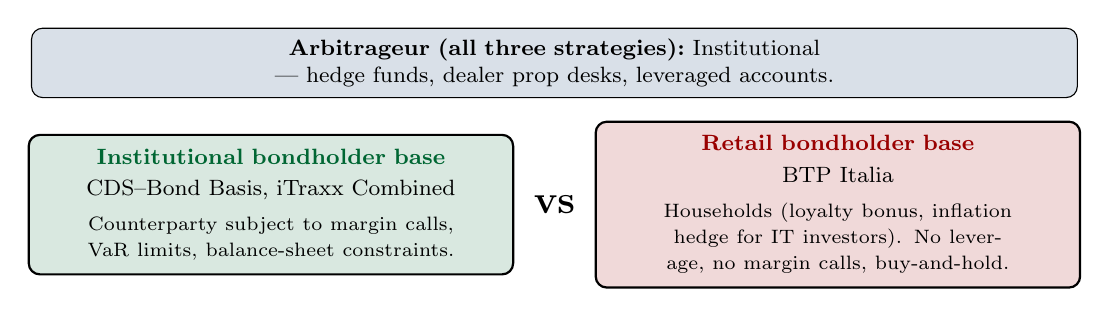
\begin{tikzpicture}[every node/.style={font=\footnotesize}]

% Header row: "Arbitrageur" — same for all 3 strategies
\node[draw, rounded corners, fill=myblue!15, text width=13cm, align=center,
      inner sep=4pt] at (0, 1.8) {%
  \textbf{Arbitrageur (all three strategies):}\ %
  Institutional --- hedge funds, dealer prop desks, leveraged accounts.
};

% Bottom row: "Bondholder base" -- 2 boxes, WIDER and SHORTER
\node[draw, rounded corners, thick, fill=mygreen!15, text width=5.8cm,
      align=center, inner sep=5pt] (inst) at (-3.6, 0.0) {%
  \textbf{\color{mygreen}Institutional bondholder base}\\[2pt]
  CDS--Bond Basis, iTraxx Combined\\[3pt]
  \scriptsize Counterparty subject to margin calls, VaR limits, balance-sheet constraints.
};

\node[draw, rounded corners, thick, fill=myred!15, text width=5.8cm,
      align=center, inner sep=5pt] (ret) at (3.6, 0.0) {%
  \textbf{\color{myred}Retail bondholder base}\\[2pt]
  BTP~Italia\\[3pt]
  \scriptsize Households (loyalty bonus, inflation hedge for IT investors). No leverage, no margin calls, buy-and-hold.
};

\node[font=\Large] at (0, 0.0) {\textbf{vs}};


\end{tikzpicture}

\vspace{0.30cm}

\textbf{Why this matters} (\citealp{brunnermeier2009market} +
\citealp{vayanos2021preferred}):
\begin{itemize}\itemsep=0.04cm\footnotesize
  \item \hltb{Institutional bondholder pair}: stress $\to$ VaR spikes $\to$
        risk budget exhausted $\to$ \emph{both} bondholders + arbitrageurs unwind.
  \item \hltb{Retail bondholder}: insulated from funding shocks
        $\to$ no forced selling $\to$ basis remains open for arbitrageurs who
        can still deploy capital.
\end{itemize}

\vspace{0.10cm}
\centering
\hlt{Identification:} \emph{if co-movement were driven by macro, all
three would move in the same direction regardless of \emph{who holds} the bond.}

\end{frame}


%------------------------------------------------------------------------------
% SLIDE 3 — P1: Cross-Market Correlation
%------------------------------------------------------------------------------
\begin{frame}[t]{P1: Cross-Market Correlation}
\small

\textit{Pearson correlations of mispricing changes $\Delta m_{i,t}$, unconditional. HAC inference.}

\vspace{0.30cm}

\input{../results/tables/RQ3_Slide_P1_Correlations.tex}

\vspace{0.40cm}

\begin{itemize}\itemsep=0.06cm\footnotesize
  \item \hlt{Within institutional pair} (CDS--Bond $\leftrightarrow$ iTraxx):
        positive correlation $\Rightarrow$ consistent with a common pool of dealer capital.
  \item \hltb{Across investor bases} (BTP~Italia pairs):
        negative correlation $\Rightarrow$ first signal of segmentation.
  \item Foundational anchor: \citet{duffie2010presidential} catastrophe-insurance
        analogy + \citet{brunnermeier2009market} commonality of liquidity (Prop.\ 6(i)).
\end{itemize}

\end{frame}


%------------------------------------------------------------------------------
% SLIDE 4 — P2: Stress Amplification
%------------------------------------------------------------------------------
\begin{frame}[t]{P2: Stress Amplification}
\small

\begin{minipage}[t]{0.58\textwidth}
\centering
\textbf{Regime correlations (Fig.~14):}\\[0.10cm]
\includegraphics[width=\textwidth,keepaspectratio]{../results/rq3_duffie/figures/C1_regime_correlations_bar_slide.pdf}
\end{minipage}\hfill
\begin{minipage}[t]{0.40\textwidth}
\vspace{0pt}
\textbf{Interaction $\hat\beta_1$:}\\[0.05cm]
{\scriptsize $\Delta m_i = \beta_0 \Delta m_j + \beta_1 (\Delta m_j \times z_t) + \gamma z_t + \varepsilon$}\\[0.10cm]
\input{../results/tables/RQ3_Slide_P2_Interaction.tex}
\end{minipage}

\vspace{0.30cm}

\begin{itemize}\itemsep=0.05cm\footnotesize
  \item \hlt{Institutional pair (CDS--Bond $\leftrightarrow$ iTraxx)}:
        $\rho$ rises monotonically LOW $\to$ HIGH $\Rightarrow$ \emph{commonality of fragility}
        \citep[Prop.\ 6(ii)]{brunnermeier2009market}.
  \item \hltb{Cross-base pairs (BTP $\leftrightarrow$ inst.)}:
        deeper negative correlation in HIGH (with sign reversal for BTP$\leftrightarrow$iTraxx) $\Rightarrow$ \emph{flight to quality}
        \citep[Prop.\ 6(iv)]{brunnermeier2009market}.
  \item Interaction $\beta_1$ confirms continuous stress amplification with sign asymmetry.
\end{itemize}

\end{frame}


%------------------------------------------------------------------------------
% SLIDE 5 — P3: Lead-Lag Transmission
%------------------------------------------------------------------------------
\begin{frame}[t]{P3: Lead-Lag Transmission}
\small

\textit{$\Delta m_{i,t} = \alpha + \sum_{j \neq i}\sum_{l=0}^{2} \beta_{j,l}\,\Delta m_{j,t-l} + \varepsilon_t$
\,---\, design of \citet{fleckenstein2014tips}.}

\vspace{0.25cm}

\input{../results/tables/RQ3_Slide_P3_SpanningGranger.tex}

\vspace{0.30cm}

\begin{itemize}\itemsep=0.05cm\footnotesize
  \item \hlt{True lead-lag}: only iTraxx$_{t-1}$ predicts the CDS--Bond basis ($\hat\beta=+0.71^*$). Other significant terms (CDS--Bond$\to$BTP, BTP$\to$CDS--Bond) are contemporaneous.
  \item \hltb{Direction (Granger)}: iTraxx Granger-causes both --- BTP~Italia ($p\!=\!0.007$) and the CDS--Bond basis ($p\!=\!0.011$); neither reverse direction is significant.
  \item \hlt{Hierarchy}: iTraxx (most liquid) $\to$ CDS--Bond $\to$ BTP~Italia, consistent with cross-strategy capital reallocation of \citet{mitchell2012arbitrage}.
\end{itemize}

\end{frame}


%------------------------------------------------------------------------------
% SLIDE 6 — P4 (NEW): Persistence Reflects Funding-Dependence
%------------------------------------------------------------------------------
\begin{frame}[t]{P4: Persistence Reflects Funding-Dependence}
\small

\textit{$m_{i,t} = c_i + \phi_i\,m_{i,t-1} + u_{i,t}$, monthly mispricing levels.
Half-life $h^* = \ln(0.5) / \ln(\phi_i)$.}

\vspace{0.30cm}

\input{../results/tables/RQ3_Slide_P4_Persistence.tex}

\vspace{0.40cm}

\begin{itemize}\itemsep=0.05cm\footnotesize
  \item \hlt{CDS--Bond is the most persistent} (half-life $\approx 3$ months): the only strategy that requires \emph{continuous repo financing} of the cash bond on dealer balance sheets \citep{boyarchenko2016trends}.
  \item \hlt{BTP~Italia and iTraxx mean-revert faster and are essentially identical} (half-life $\approx 2$ months at $\phi \approx 0.73$): the two less funding-intensive strategies are statistically indistinguishable from each other in monthly persistence.
  \item Persistence is segregated by \hltb{funding-dependence of execution}: only the strategy requiring continuous repo financing of a cash bond stands apart from the two derivative-based bases.
\end{itemize}

\end{frame}

%------------------------------------------------------------------------------
% SLIDE 7 — P5: Common Factor = Intermediary, NOT Macro
%------------------------------------------------------------------------------
\begin{frame}[t]{P5: Common Factor $\to$ Intermediary Capital, \emph{not} Macro}
\small

\input{../results/tables/RQ3_Slide_P5_PC1_Funding.tex}

\vspace{0.25cm}

\begin{itemize}\itemsep=0.06cm\footnotesize
  \item \hlt{Panel A}: all four intermediary proxies significant with the predicted sign $\Rightarrow$ direct empirical content of \citet{duffie2010presidential} and Prop.\ 6(i) of \citet{brunnermeier2009market}.
  \item \hltb{Panel C (placebo)}: \emph{none} of the four macro proxies is significant; model not jointly significant ($F$-test $p\!=\!0.23$) $\Rightarrow$ confirms common factor is balance-sheet, not macro.
\end{itemize}

\end{frame}

%------------------------------------------------------------------------------
% SLIDE — All Five Predictions Find Support
%------------------------------------------------------------------------------
\begin{frame}[t]{All Five Predictions Find Support}
\small

\input{../results/tables/RQ3_Slide_Mapping_Scorecard.tex}

\end{frame}

%------------------------------------------------------------------------------
% SLIDE 9 — Why Persist (closing)
%------------------------------------------------------------------------------
\begin{frame}[t]{Why Do These Arbitrages Persist?}
\small

\textbf{Three reinforcing mechanisms:}

\begin{itemize}\itemsep=0.20cm
  \item \hlt{Regulatory cost of intermediary capacity} \citep{boyarchenko2016trends}: \\
        post-crisis SLR and Basel III have permanently raised the cost of dealer balance sheet, lifting the equilibrium level of basis trades --- evident in the high persistence of CDS--Bond ($\phi = 0.79$, P4).

  \item \hlt{Slow-moving capital across strategies} \citep{duffie2010presidential, mitchell2012arbitrage}: \\
        capital reallocates across the dealer network on a horizon of several months. iTraxx adjusts first, BTP~Italia last (P3), and the common factor is intermediary balance-sheet, not macro fundamentals (P5).

  \item \hltb{Investor-base segmentation as a structural feature}: \\
        BTP~Italia retail bondholders generate a preferred-habitat \citep{vayanos2021preferred} structurally insulated from institutional unwinding --- the basis remains open for arbitrageurs who can deploy capital, but the funding-dependence of execution determines who can.
\end{itemize}

\vspace{0.20cm}

\centering
\textcolor{myblue}{\textbf{Bottom line:} the geography of slow-moving capital is determined not by
asset-class labels but by the network of intermediaries that service these
markets --- and ultimately by who holds the bonds.}

\end{frame}


\end{document}
